\documentclass[tikz,border=3mm]{standalone}
\usepackage[T1]{fontenc}
\usepackage{lmodern}
\usetikzlibrary{arrows.meta,calc}
\definecolor{concrete}{HTML}{EAF3FB}
\definecolor{abstract}{HTML}{FFF3C4}
\definecolor{operation}{HTML}{E2F1EB}
\definecolor{field}{HTML}{FBE5CE}
\definecolor{purevirtual}{HTML}{A33131}
\definecolor{ink}{HTML}{444444}
\begin{document}
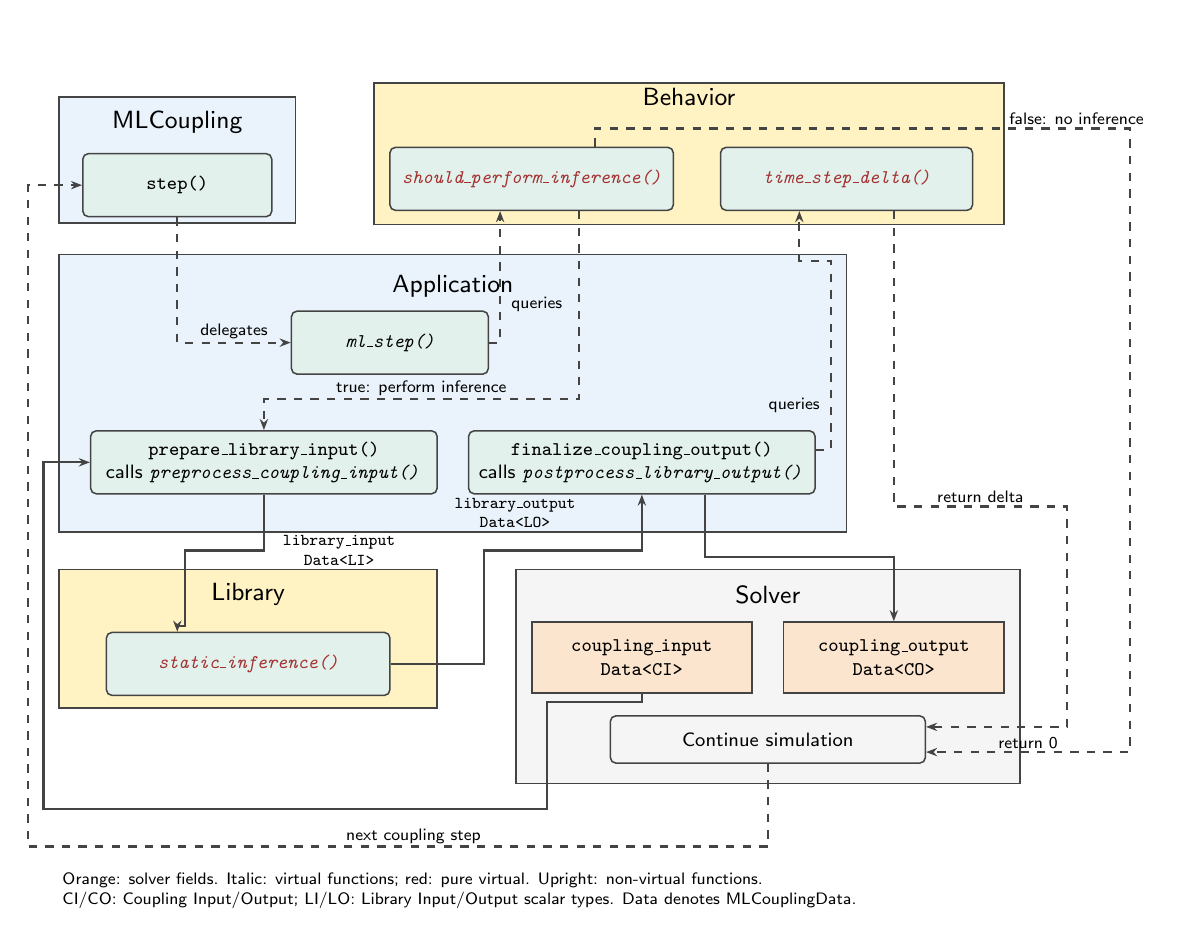
\begin{tikzpicture}[
  x=1mm,y=.8mm,font=\sffamily\fontsize{9}{10.5}\selectfont,
  class/.style={draw=ink,line width=.65pt,fill=concrete,
    minimum width=30mm,minimum height=9mm,align=center,inner sep=2pt},
  abstract/.style={class,fill=abstract},
  operation/.style={draw=ink,line width=.55pt,fill=operation,
    rounded corners=2pt,minimum height=8mm,align=center,inner sep=2pt,
    font=\sffamily\fontsize{7}{8.5}\selectfont},
  virtual/.style={font=\sffamily\fontsize{7}{8.5}\selectfont\itshape},
  purevirtual/.style={virtual,text=purevirtual},
  field/.style={class,fill=field,minimum width=28mm,
    font=\sffamily\fontsize{7}{8.5}\selectfont},
  relation/.style={draw=ink,line width=.8pt},
  flow/.style={relation,-{Stealth[length=4pt,width=3pt]}},
  control/.style={flow,dashed},
  label/.style={font=\sffamily\fontsize{6}{7}\selectfont,inner sep=1pt,align=center},
  note/.style={anchor=west,font=\sffamily\fontsize{7}{8.5}\selectfont,inner sep=0pt}
]
\path[use as bounding box] (78,4) rectangle (222,-137);

% Ordinary static orchestration; all bends use projections or matched anchors.
\node[class,minimum height=16mm] at (97,-17) {};
\node at (97,-11) {MLCoupling};
\node[operation,minimum width=24mm] (step) at (97,-21) {\texttt{step()}};

\node[abstract,minimum width=80mm,minimum height=18mm] at (162,-16) {};
\node at (162,-7) {Behavior};
\node[operation,purevirtual,minimum width=36mm] (decision) at (142,-20)
  {\texttt{should\_perform\_inference()}};
\node[operation,purevirtual,minimum width=32mm] (delta) at (182,-20) {\texttt{time\_step\_delta()}};

\node[class,minimum width=100mm,minimum height=35.2mm] at (132,-54) {};
\node at (132,-37) {Application};
\node[operation,virtual,minimum width=25mm] (mlstep) at (124,-46) {\texttt{ml\_step()}};
\node[operation,minimum width=44mm] (pre) at (108,-65)
  {\texttt{prepare\_library\_input()}\\calls \textit{\texttt{preprocess\_coupling\_input()}}};
\node[operation,minimum width=44mm] (post) at (156,-65)
  {\texttt{finalize\_coupling\_output()}\\calls \textit{\texttt{postprocess\_library\_output()}}};
\draw[control] (step.south) |- node[label,pos=.75,above] {delegates} (mlstep.west);
\draw[control] (mlstep.east) -- (138,-46) -- ($(decision.south)+(-4,0)$);
\node[label,anchor=west] at (139,-40) {queries};
\draw[control] ($(decision.south)+(6,0)$) -- (148,-55)
  -- node[label,above] {true: perform inference} (108,-55) -- (pre.north);

% Library and Solver share their top edge; solver fields are CI/CO, not LI/LO.
\node[abstract,minimum width=48mm,minimum height=17.6mm] at (106,-93) {};
\node at (106,-86) {Library};
\node[operation,purevirtual,minimum width=36mm] (infer) at (106,-97) {\texttt{static\_inference()}};
\draw[flow] (pre.south) -- (108,-79) -- (98,-79)
  -- (98,-91) -| ($(infer.north)+(-9,0)$);
\node[label,anchor=west] at (110,-79) {\texttt{library\_input}\\\texttt{Data<LI>}};
\draw[flow] (infer.east) -- (136,-97) -- (136,-79)
  -- (156,-79) -- (post.south);
\node[label,anchor=east] at (148,-73) {\texttt{library\_output}\\\texttt{Data<LO>}};

\node[class,fill=gray!8,minimum width=64mm,minimum height=27.2mm] (solver) at (172,-99) {};
\node at (172,-86) {Solver};
\node[field] (ci) at (156,-96) {\texttt{coupling\_input}\\\texttt{Data<CI>}};
\node[field] (co) at (188,-96) {\texttt{coupling\_output}\\\texttt{Data<CO>}};
\node[operation,fill=gray!8,minimum width=40mm,minimum height=6mm] (advance) at (172,-109)
  {Continue simulation};
\draw[flow] (ci.south) -- (156,-103) -- (144,-103)
  -- (144,-120) -- (80,-120) |- (pre.west);
\draw[flow] ($(post.south)+(8,0)$) -- (164,-80) -| (co.north);
\draw[control] (advance.south) -- (172,-126) -- (78,-126) |- (step.west);
\node[label,above] at (127,-126) {next coupling step};

\draw[control] ($(decision.north)+(8,0)$) -- (150,-12)
  -- node[label,pos=.9,above] {false: no inference} (218,-12)
  |- node[label,pos=.75,above] {return 0} ($(advance.east)+(0,-2)$);
\draw[control] ($(post.east)+(0,2)$) -| (180,-33) -| ($(delta.south)+(-6,0)$);
\node[label,anchor=east] at (179,-56) {queries};
\draw[control] ($(delta.south)+(6,0)$) -- (188,-72)
  -- node[label,above] {return delta} (210,-72)
  |- ($(advance.east)+(0,2)$);

\node[label,anchor=west,align=left] at (82,-133) {
  Orange: solver fields. Italic: virtual functions; red: pure virtual. Upright: non-virtual functions.\\
  CI/CO: Coupling Input/Output; LI/LO: Library Input/Output scalar types. Data denotes MLCouplingData.
};
\end{tikzpicture}
\end{document}
